\chapter{Related work}
The internet traffic explosion started in the mid-90s induced the creation of massive datasets. Processing very large amount of data, even though can be conceptually straightforward, actually means many computations that have to be distributed across hundreds or thousands of machines in order to finish in a reasonable amount of time. In early 2000s, the developer had the burden to write complex applications responsible for parallelizing the computation, distributing the data, and handling possible failures. As a reaction to this complexity, Google in 2004 published a paper describing a novel programming model for processing large datasets named MapReduce \cite{googlemapreduce}. MapReduce provides an abstraction that allows the developer to focus on the computation he/she wants to express hiding the details of parallelization, fault-tolerance, data distribution and load balancing in a framework. The MapReduce framework takes advantage of the Google File System \cite{googlefilesystem}: a distributed file system that uses replication to provide availability and reliability on top of commodity unreliable hardware. The open source community, inspired by the Google MapReduce programming model, created Hadoop \cite{hadooponline} and HDFS \cite{hadoophdfs}. The Hadoop release boosted the growth of the big data analysis field and created new scenarios and new type of applications that were very tough to realize with previous existing tools. From that moment on, a lot of effort has been put in realizing more efficient and high-performance technologies for collecting, aggregating and analyzing huge amount of data.

In this chapter we will discuss some of the technologies and architectures that can be used in order to process large amount of data generated by (IoT) sensors, possibly in real-time.

\section{Batch-Mode architecture}
Google MapReduce and Hadoop are designed to be executed on top of clusters of computing nodes. The first releases of Hadoop integrated the cluster resource management with the data processing engine itself (Hadoop MapReduce). In 2012, Hadoop 2.0 was released \cite{hadooponline} and it introduced YARN \cite{yarn}; Apache Yet Another Resource Negotiator (YARN) decouples the programming model from the resource management infrastructure and the users' applications scheduling. In general, we can think to YARN as a distributed operating system that is capable of managing a cluster of machines and scheduling users' applications on the available resources. Furthermore, it provides an API that can be used to develop any generic distributed application. Hence, different computing frameworks that address different application requirements have been built on top of YARN (e.g. the general purpose Apache Spark \cite{apachesparkonline}, Apache Giraph \cite{apachegiraphonline} for iterative graph processing, etc.). 

 \begin{figure}[ht!]
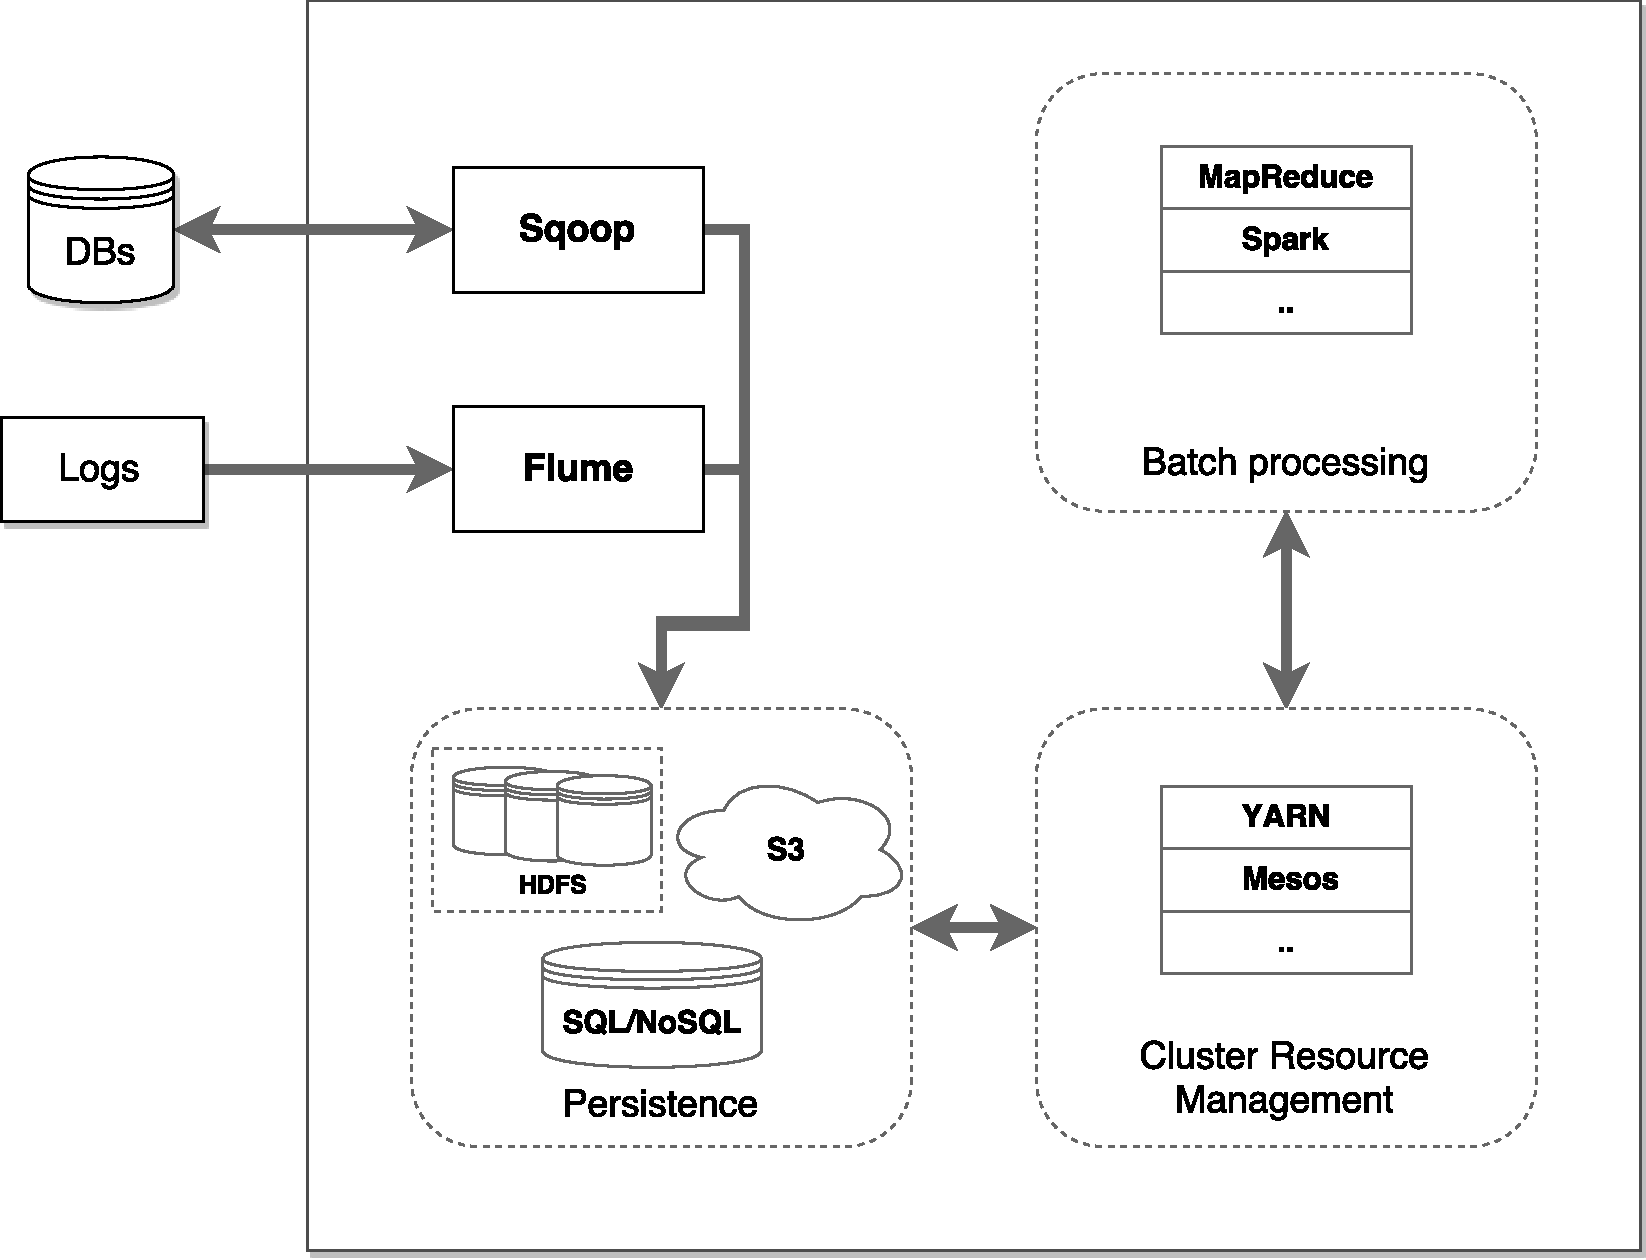
\includegraphics[width=1\textwidth]{images/batch_architecture.pdf}
 \caption{Classic big data batch architecture}
\label{fig:batch_architecture}
\end{figure}

A big data application usually has a well defined architecture, no matter the computing framework it uses and whether or not it runs on top of YARN or on another cluster management system (e.g. Apache Mesos  \cite{apachemesosonline}, Kubernetes \cite{kubernetesonline}, in the cloud using Amazon Elastic Map Reduce (EMR) \cite{amazonemronline}). The \emph{classic} big data architecture for processing large amount of structured or unstructured data is named \emph{batch architecture} \cite{philosophydistributeddata, fastdataarchitecture, streamingbigdataprocessinginclouds}. The typical big data batch architecture consists of the following components or layers (see Figure \ref{fig:batch_architecture}):
\begin{itemize}
\item	 \emph{Data ingestion layer}. The data ingestion layer can be used to move data that can come from different sources into the persistence tier. The data ingestion layer can take advantage of special-purpose services such as Apache Flume \cite{apacheflumeonline} for log aggregation or Apache Sqoop \cite{apachesqooponline} for interoperating with databases.
\item \emph{Data persistence layer}. The data persistence layer is responsible of storing and indexing final as well intermediate datasets. This tier can store large amount of data using one of the next-generation database systems. In fact, the Dynamo \cite{dynamo} paper accelerated interest in NoSQL systems and many NoSQL database emerged such as Apache Cassandra \cite{apachecassandraonline} or MongoDB \cite{mongodbonline}. Furthermore, the CAP theorem emerged as a way of understanding the trade-offs between consistency and availability of service in distributed systems when a network partition occurs. For the always-on applications, it often made sense to accept \emph{eventual consistency} in exchange for a greater availability \cite{fastdataarchitecture}. In big data application, database systems are often used when row-level access (e.g. CRUD operations) is required \cite{fastdataarchitecture}.

In order to store large datasets, the data persistence layer can also use a distributed file system or object store, such as HDFS or Amazon S3 \cite{awss3online}. These systems offers lower cost per GB storage compared to databases and more flexibility for data formats \cite{fastdataarchitecture}. However, they are best used when scans are the dominant access pattern, rather than CRUD operations. 
\item  \emph{Cluster resource management}. The cluster distributed operating system.
\item  \emph{Data Processing layer}. The data analysis jobs written in Hadoop MapReduce, Spark, or other tools submitted to the cluster resource manager.
\end{itemize}

A typical big data application can be built as a \emph{workflow}, a directed graph of distributed computing jobs \cite{bigdataatlinkedin}. Each job reads one or more input datasets from the persistent storage and produces one or more output datasets. In MapReduce, if the application requires data reuse between computations (e.g. between two jobs) the intermediate result is also written to an external stable storage system. This can incur substantial overheads due to data replication, disk I/O, and serialization, which can dominate application execution times. Recognizing this problem, researchers have developed specialized frameworks for some applications that require data reuse. These frameworks only support specific computation patterns and perform data sharing implicitly for these patterns. Eventually, the general purpose computing framework Apache Spark \cite{apachespark} was released. Spark is the first system that allows a general-purpose programming language to be used at interactive speeds for in-memory data mining on clusters \cite{apachespark}. Spark is based on the concept of resilient distributed datasets (RDDs) \cite{apachesparkrdd} that enables efficient data reuse in a broad range of applications. The RDD abstraction allows users to explicitly persist intermediate results in memory, control the data partitioning to optimize the data placement, and manipulate them using a rich set of operators. Even though Spark increased the interactivity of many big data applications and tools, a typical job in batch-mode can last from few minutes to several hours. In fact, in classic batch-mode, data is collected and stored in the persistent storage layer and once in a while (e.g. every hour, once per day) the data is processed through one or more batch jobs. The high-latency imposed by the batch architecture is not suitable for real-time applications in which data should be computed as it is generated, in an incremental fashion.

\section{Real-time streaming architecture}
Recently, many big data real-time applications emerged such as detecting fraudulent financial activity as it happens or optimizing e-commerce search results in real-time. These kinds of applications process unbounded datasets and potentially infinite \emph{streams} of data, and they are often  referred as real-time streaming applications. A real-time streaming application is usually backed by a distributed, high-performance and always available architecture. There are many streaming systems and ways of doing streaming, and everything is evolving quickly. Figure \ref{fig:lambda_architecture} represents a real-time streaming architecture. This architecture is also called Lambda architecture \cite{fastdataarchitecture, lambdaarchitecturecosteffective, alljoynlambda} and it was designed by Nathan Marz based on his experience working on distributed data processing systems at Twitter. The Lambda architecture is essentially composed by two computing \emph{layers} or \emph{paths} that can be realized using various big data technologies:
\begin{itemize}
\item \emph{A batch (or offline) layer}. The batch layer aims at perfect accuracy by being able to process all available data when generating a computing result. This means it can fix any errors by recomputing based on all the available historical data.

\item \emph{A speed (or online) layer}. The purpose of this layer is minimize latency by doing real time calculations as the data arrives into the system. The output of this layer does not guarantee accuracy and completeness as the one eventually produced by the batch layer. The result of this layer can be replaced when the batch layer process a consistent output for the same input data (if necessary).
\end{itemize}

The Lambda architecture can also involve a third layer named \emph{serving layer}. It combines the output from the batch and speed layers and it is used to respond to ad-hoc queries.

In the following sections we will discuss and highlight the core components of the real-time streaming architecture and what makes this architecture different from the batch-mode.

 \begin{figure}[ht!]
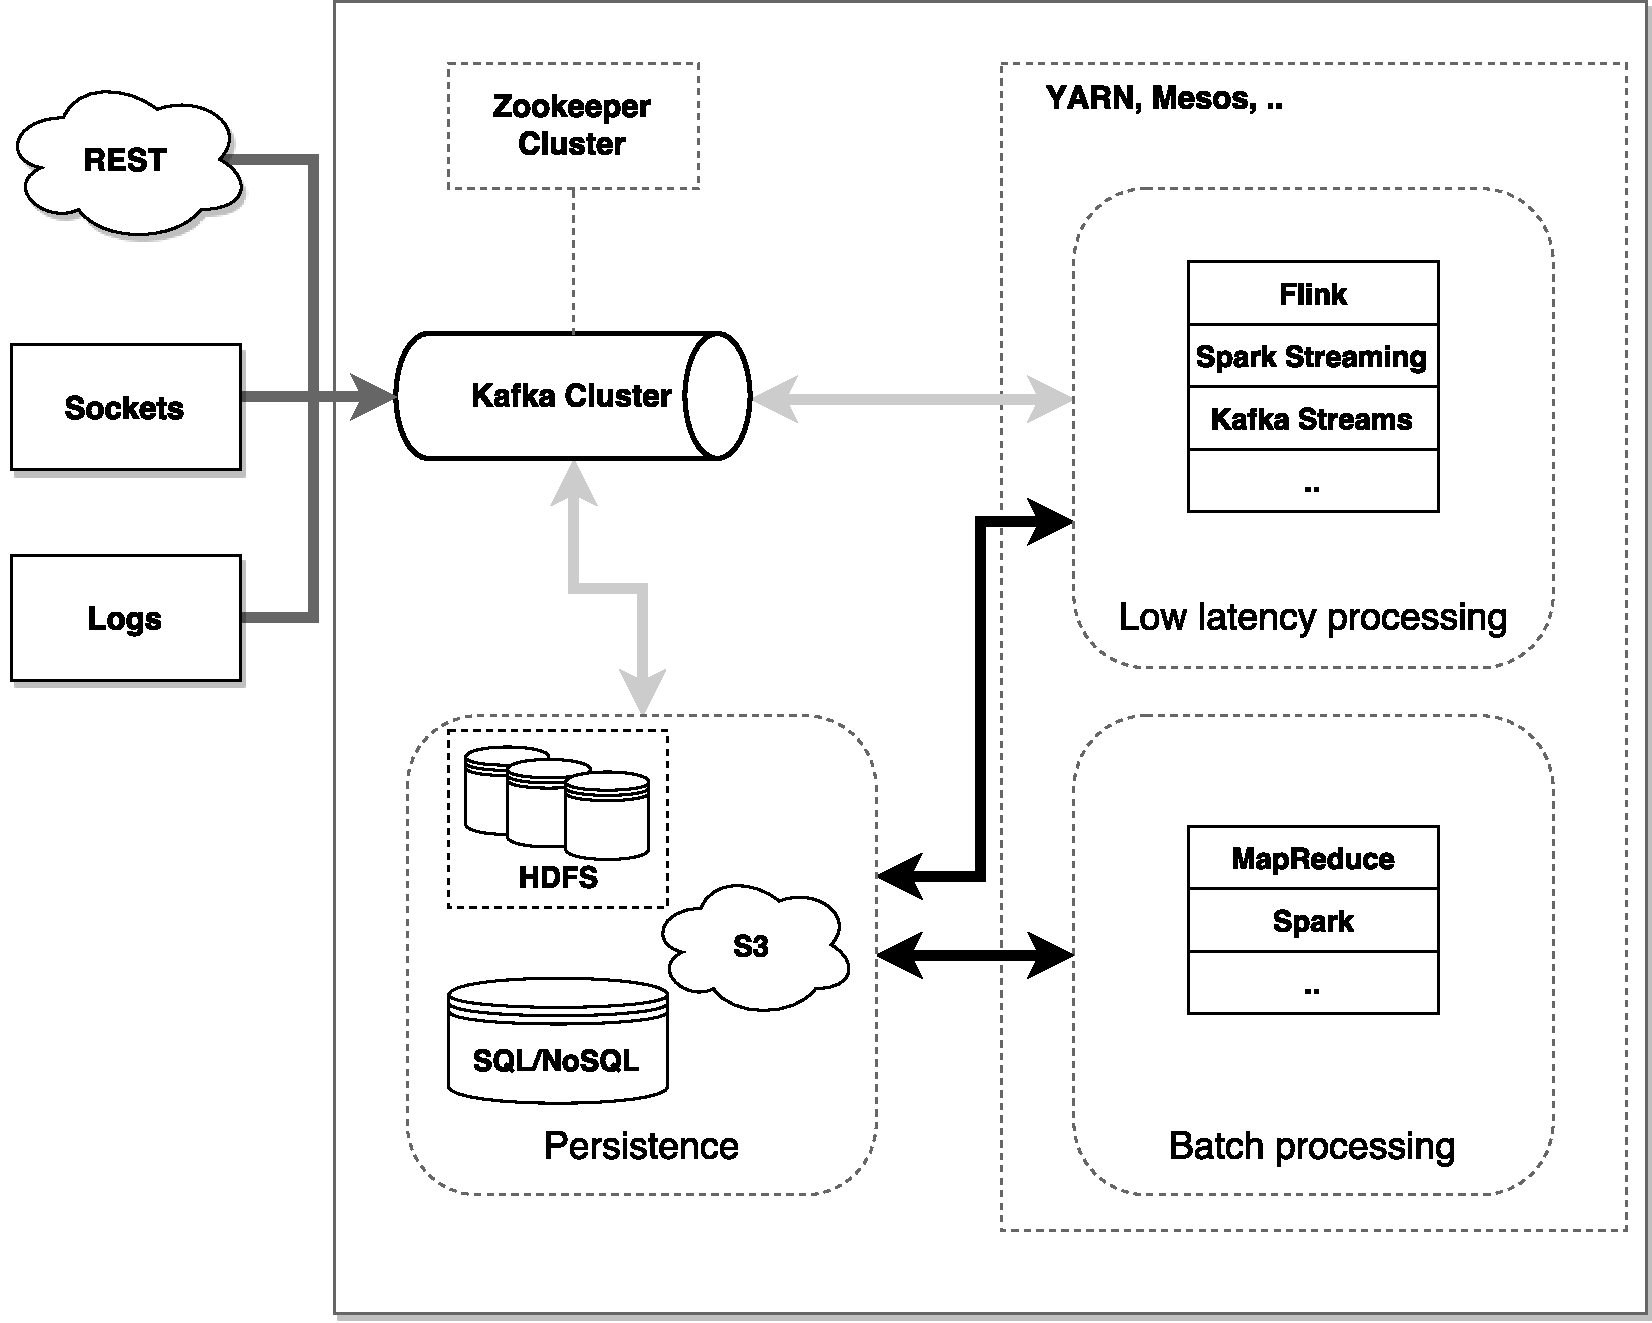
\includegraphics[width=1\textwidth]{images/streaming_architecture.pdf}
 \caption{The Lambda architecture}
\label{fig:lambda_architecture}
\end{figure}

\subsection{Distributed message broker}
Streams of data can arrive into the system over sockets from other servers within the environment or from outside. For example, data such as telemetry values from IoT devices or social network feeds coming from the Twitter “firehose” can be continuously \emph{polled} and ingested into the system. Data could also flow into the system via REST or via continuously updated log files \cite{fastdataarchitecture}. This large streams of data can be ingested in the system through a message queue. Message queues are \emph{first-in, first-out} (FIFO) data structures, which is also the natural way to process data that come in streaming. Message queues/brokers organize the ingested data into user-defined \emph{topics}: each topic has its own queue. Producers/publishers send information to the message queue at a specific topic; a consumer/subscriber receives automatic messages every time there is a new update in a topic it is a subscriber. This promotes scalability through parallelism (each topic has its own queue), and it also allows producers and consumers to focus only on topics of interest. A distributed, efficient and reliable message broker is the backbone of a high-performance streaming architecture \cite{fastdataarchitecture}. It provides scalable, durable and temporary storage; furthermore, it disseminates data to the different internal components as the data flow into the system. The most popular message broker system used within a streaming architecture is Apache Kafka \cite{apachekafkaonline}. 
\subsubsection{Apache Kafka}
Apache Kafka is a massively scalable publish/subscribe message queue architected as a distributed transaction \emph{log}. It benefited from years of production use and development at LinkedIn, where it started. In September 2015, the LinkedIn’s deployment of Apache Kafka surpassed 1.1 trillion messages per day \cite{fastdataarchitecture}.  

A Kafka topic is divided into \emph{partitions}: messages within a partition are totally ordered. Topics partitioning is necessary in order to provide \emph{horizontal scalability}: different partitions can reside on different machines and no coordination across partitions is required. The assignment of messages to partitions may be random, or it may deterministic based on a key \cite{philosophydistributeddata}. A Kafka partition is also known as a \emph{log}, since it resembles a database’s transaction commit log \cite{philosophydistributeddata}: when a new message is published to a certain topic, it is appended to the end of the log. \emph{Fault-tolerance} is guaranteed replicating each partition across multiple Kafka nodes. One of the replicated partition is elected as \emph{leader} and it is responsible for handling all reads and writes of messages for that partition. All the updates to the partition are then synchronously propagated from the leader to a configurable number of replicas. On leader failure, one of the \emph{in-sync} replicas is chosen as the new leader \cite{philosophydistributeddata}. 

In Kafka, a message is composed by a \emph{key} and a \emph{value}. When a message is published to a certain topic, the Kafka broker assigns an \emph{offset} to that message, which is a per-partition monotonically increasing sequence number. A Kafka consumer application reads all the messages in a topic partition sequentially. For each partition, the client keeps track of the offset up to which it has seen messages, and it continuously polls the brokers waiting for the arrival of new messages with a greater offset .The offset is periodically checkpointed to stable storage; if a consumer client application crashes and restarts, it resumes reading from its most recently checkpointed offset \cite{philosophydistributeddata}. In Kafka, messages are not deleted when read, so any number of readers can ingest all the messages in a topic. In fact, Kafka deletes the oldest message using a user-specified retention time (which by default is set to seven days) or a maximum number of bytes in the queue (the default is unbounded). A combination of the two approaches is also possible \cite{fastdataarchitecture}.

Kafka as a distributed system works in combination with Apache Zookeeper \cite{apachezookeeperonline}. Zookeeper is used for tasks requiring consensus, such as leader election, and for storage of some state information.


% there is no ordering guarantee, instead, across different partitions.  and messages within a partition are totally ordered. There is no ordering
% guarantee across different partitions. 
%The


\subsection{Low latency processing}
One of the core components of a real-team streaming architecture is the low latency streaming processing engine. These are scalable distributed systems that continuously process, aggregate and analyze unbounded streams of data. In the Lambda architecture, they serve as \emph{speed layer}. The computations of these systems are usually modelled as Direct Acyclic Graph (DAG) topologies. Many streaming computing technologies have arosen such as Apache Spark Streaming \cite{apachesparkstreamingonline}, Flink \cite{apacheflinkonline}, Storm (and Trident) \cite{apachestormonline}, Samza \cite{apachesamzaonline}, Heron \cite{herononline}, Kafka Streams \cite{kafkastreamsonline} and many others. All these systems usually run on top of a clustering system such as YARN or Mesos. However, these frameworks do have some differences in the underlying architecture that can mean different performance in terms of throughput, latency and accuracy. We will discuss the peculiarities and architectural characteristics of these systems in the next chapter. For now, we can think to a streaming engine as a processing framework that is capable of processing huge volume of data continuously as the data is flowing through the system. The latency of these systems can usually vary from hundreds of milliseconds to few seconds. 

In a streaming environment, a low latency computing engine process data that come from a distributed message broker such as Apache Kafka and then the output is written back to Kafka. The stream processing results can also be saved to the persistent storage. Potentially, the input data of the streaming computation can also be ingested from the persistent storage, although this imposes higher latency than streaming through Kafka.

\subsection{Batch processing}
A streaming architecture usually has also support for a traditional batch processing system. In fact, as we already mentioned, the core concept behind the so called Lambda architecture is to handle massive quantities of data by taking advantage of both batch and stream processing methods. A batch processing framework acts as \emph{batch (or offline) layer}. This layer can adopt any traditional big data processing framework that are commonly used in the batch architecture and they are used to perform expensive calculations with data coming from the persistent storage. In fact, the data coming into the system through Apache Kafka can be consumed by a streaming application running on top of a streaming engine but it can also be stored in the persistent storage layer.


\subsection{Persistence}
In the Lambda architecture, the data persistence component is basically used as in the batch-mode architecture. It can also be used as \emph{serving layer} for combining the output from the batch and speed layers.


\subsection{Streaming architectures for IoT scenarios}
In the literature, there are some example of Lambda architecture applied to the IoT scenario. In \cite{lambdaarchitecturecosteffective}, they propose a framework built in the Amazon cloud for processing large amount of data coming from smart city sensors. This architecture, designed on top of EMR, uses Amazon Kinesis \cite{amazonkinesisonline} for data ingestion; Kinesis is also used, in combination with Amazon Lambda \cite{amazonlambdaonline}, for the speed processing layer. The batch layer is realized through MapReduce jobs executed on EMR. Amazon S3 is used as persistent storage layer. 

In \cite{alljoynlambda}, they bring the Lambda architecture to the  AllJoyn framework \cite{alljoynframeworkonline}. Alljoyn is an open source project for the development of a universal software framework aimed at the interoperability among heterogeneous devices, dynamic creation of proximal networks and execution of distributed applications. However, AllJoyn does not scale well because it does not support communications among devices belonging to different broadcast domains (i.e. belonging to different subnets) and it does not provide any feature for the storage and real-time analytics of huge amount of data. In \cite{alljoynlambda}, they overcome this limitation integrating the AllJoyn framework with Apache Storm for real-time stream processing and MongoDB for the massively storage.

In the next chapters we are going to describe how the current Cowbird implementation can be integrated with a scalable and distributed real-time streaming architecture.









